%%%%%%%%%%%%%%%%%%%%%%%%%%%%%%%%%%%%%%%%%
% University/School Laboratory Report
% LaTeX Template
% Version 3.1 (25/3/14)
%
% This template has been downloaded from:
% http://www.LaTeXTemplates.com
%
% Original author:
% Linux and Unix Users Group at Virginia Tech Wiki 
% (https://vtluug.org/wiki/Example_LaTeX_chem_lab_report)
%
% License:
% CC BY-NC-SA 3.0 (http://creativecommons.org/licenses/by-nc-sa/3.0/)
%
%%%%%%%%%%%%%%%%%%%%%%%%%%%%%%%%%%%%%%%%%

%----------------------------------------------------------------------------------------
%	PACKAGES AND DOCUMENT CONFIGURATIONS
%----------------------------------------------------------------------------------------

\documentclass{article}

\usepackage{float}
\usepackage{listings}

\usepackage[version=3]{mhchem} % Package for chemical equation typesetting
\usepackage{siunitx} % Provides the \SI{}{} and \si{} command for typesetting SI units
\usepackage{graphicx} % Required for the inclusion of images
\usepackage{amsmath} % Required for some math elements 
\setlength\parindent{0pt} % Removes all indentation from paragraphs
\usepackage{mathtools}
\DeclarePairedDelimiter{\floor}{\lfloor}{\rfloor}
\renewcommand{\labelenumi}{\alph{enumi}.} % Make numbering in the enumerate environment by letter rather than number (e.g. section 6)

%\usepackage{times} % Uncomment to use the Times New Roman font

%----------------------------------------------------------------------------------------
%	DOCUMENT INFORMATION
%----------------------------------------------------------------------------------------

\title{RTS Lab 1 Protokoll} % Title

\author{Jan Niklas Hollenbeck 735992 \\ Lukas Giesler} % Author name

\date{\today} % Date for the report

\begin{document}

\maketitle % Insert the title, author and date

% If you wish to include an abstract, uncomment the lines below
% \begin{abstract}
% Abstract text
% \end{abstract}

%----------------------------------------------------------------------------------------
%	SECTION 1
%----------------------------------------------------------------------------------------

\section{Aufgabe 1}

Calculation of Times and Deadlines in the physical world.


\subsection{Time calculations}
Formula for Speed:  $s = v*t$\\

\begin{tabular}{ll}
$s$ & distance in Meter[m]\\
$v$ & speed in meters per second [m/s]\\
$t$ & time in seconds [s]\\
\end{tabular}


\subsubsection{}
How long does it take a Car to travel the distance of \SI{1}{\meter} when travelling 30/50/100/200 km/h ?\\
Rearrange formula to get s/m: $\dfrac{1}{\dfrac{10}{36} * s * \dfrac{h}{Km}  * \dfrac{m}{s}}$\\
For s use speed in Km/h:

$30km/h = 0,12 s/m$\\
$50km/h = 0,072 s/m$\\
$100km/h = 0,036 s/m$\\
$200km/h = 0,018 s/m$\\
\subsubsection{}
How far does a missile at mach 3 fly´s in 1ms?\\
mach = 1234,8 Km/h \\
mach 3 = 3704,4 Km/h
Formular to get m/ms : $\dfrac{10}{36} * s * \dfrac{h}{Km}  * \dfrac{m}{1000ms}$\\
3704,4km/h = 1,029 m/ms

\subsubsection{}
Which distance travels a light ray in vacuum?\\
Speed of light = $3x10^8 m/s$\\
Formula to get m/ns: $s *\dfrac{m/s}{1x10^9ns}$\\
$3x10^8m/s = 0,3 m/ns$
\subsubsection{}
Formula for frequency: $ f = \dfrac{1}{T}$

\begin{tabular}{ll}
$f$ & frequency[Hz]\\
$T$ & Period time  [s]\\
\end{tabular}

$0,3m / 1,5x10^8 m/s = 2x10^-9$
$\dfrac{1}{2x10^-9}= 500mHz$

\subsubsection{}
Shannons theorem states, to sample a signal the sampling rate: $Ts$ must be smaller then the $T/2$ where T  is the Frequency of the Signal.
Otherwise it is impossible to reconstruct the original Signal.

Therefore the sampling rate for a  3,2 kHz Signal must be at least greater as 6.2 kHz.

$\floor[\big]{\dfrac{16mHz}{6,2kHz}} = 2580  Cycles $

%----------------------------------------------------------------------------------------
%	SECTION 2
%----------------------------------------------------------------------------------------

\section{ Cyclic Executive Approach}

\subsection{}
The major cycle is calculated by the Least common multiple of the Processes execution times.\\
$Lcm(25,50,100)=100$ \\
The Major cycle is thereby 100.\\
\\
The minor cycle is determined by  the smallest execution time.\\
The minor cycle is 25.
\newpage
\subsubsection{}
In the Figure \ref{fig:Bild1} the RTS for the Process Table is shown in a Linear fashion.
\begin{figure}[H] 
  \centering
     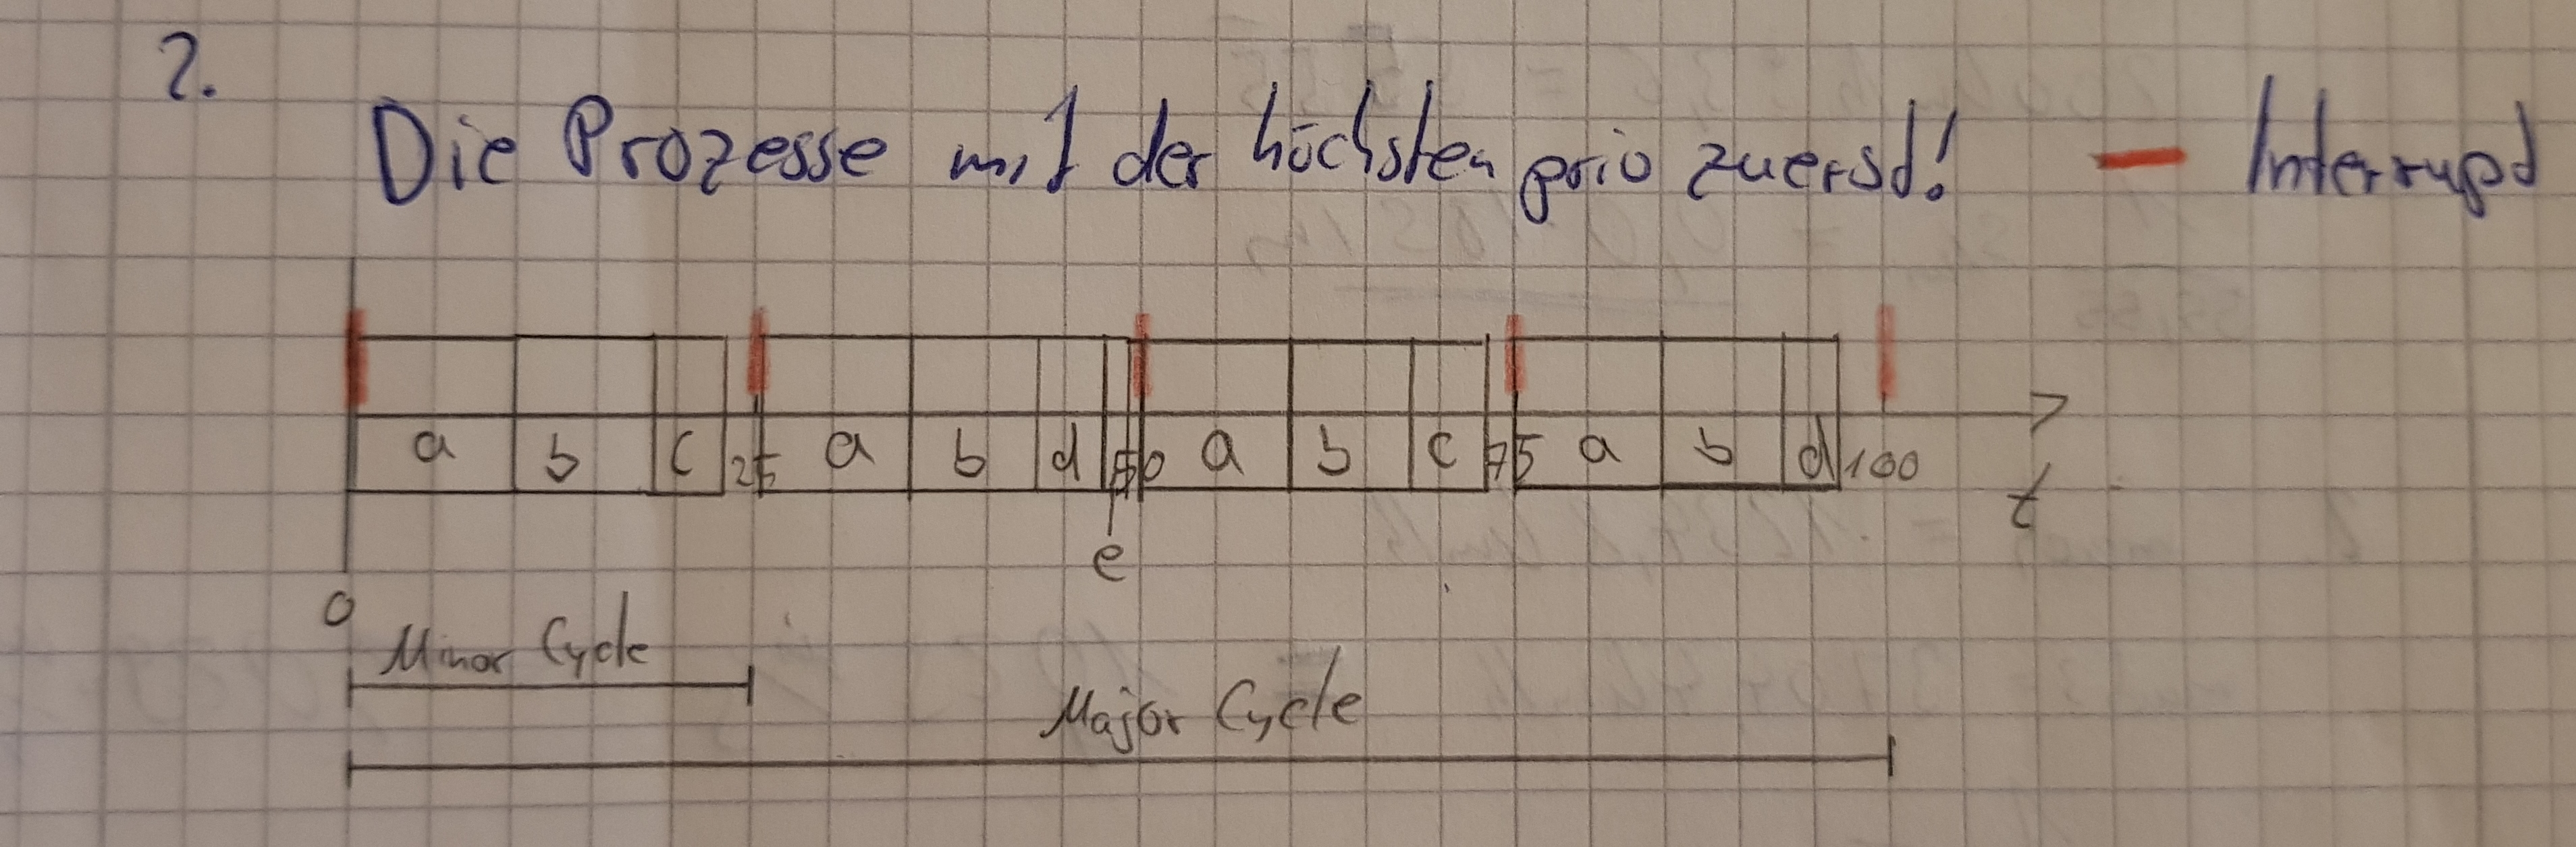
\includegraphics[width=1\textwidth]{RTS.jpg}
  \caption{RTS Graph}
  \label{fig:Bild1}
\end{figure}

\subsubsection{}
\begin{lstlisting}
loop
	wait_for_interrupt(time=0);
	call_procedure(a);
	call_procedure(b);
	call_procedure(c);
	wait_for_interrupt(time=25);
	call_procedure(a);
	call_procedure(b);
	call_procedure(d);
	call_procedure(e);
	wait_for_interrupt(time=50);
	call_procedure(a);
	call_procedure(b);
	call_procedure(c);
	wait_for_interrupt(time=75);
	call_procedure(a);
	call_procedure(b);
	call_procedure(d);
	wait_for_interrupt(time=100);
end loop;
\end{lstlisting}



\end{document}